\paragraph{Highest Concurrency:} In figure \ref{fig:concurrency} we can see the concurrency (i.e., the number of active interventions at a given time) of an example solution. The highest concurrency represents the maximum number of interventions being executed simultaneously at any time. In order to get the final score for the decision matrix, we normalize using the total number of interventions.

\begin{figure}[ht]
    \centering
    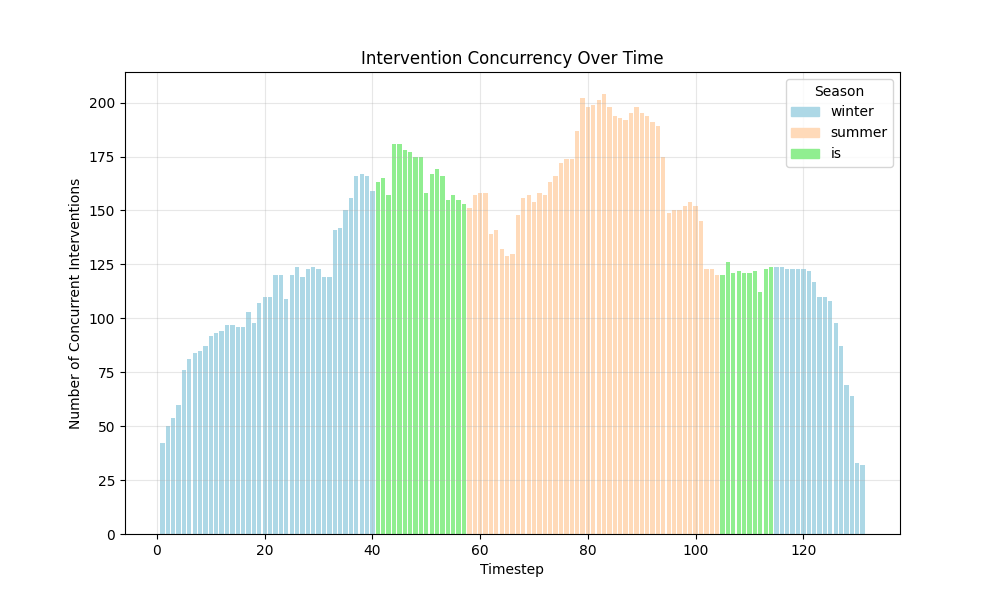
\includegraphics[width=\textwidth]{ch3/figures/Concurrency.png}
    \caption{Concurrent interventions over time for an example solution, showing the number of interventions being executed simultaneously at each time period. Colors are used to differentiate seasons.}
    \label{fig:concurrency}
\end{figure}



% \paragraph{Highest Risk:} This attribute measures the average worst-case risk across all interventions, where for each intervention we consider its maximum risk over all time periods and scenarios. Formally, we have:

% \[\operatorname{worst}^{(i,\tau)} \coleq \max_{t=1,\dots,d_{i,\tau}} \max_{s\in S} \mathrm{risk}_{s,t}^{(i,\tau)} \quad \text{where} \quad \text{highest\_risk} \coleq \frac{1}{|\mathcal{I}|}\sum_{i\in\mathcal{I}} \operatorname{worst}^{(i,\tau_i)}\]



\paragraph{Seasonality:} These are 3 attributes that indicate the proportion of total interventions active in each season (Winter, Summer, or Interseason). Note that the proportions sum to more than 1 since interventions can span multiple seasons.